\section{Introducción}

\subsection{1.1 Motivación y Contexto en Observación Terrestre}

Aunque los sensores satelitales modernos generan volúmenes de datos sin precedentes, la mayor parte de las imágenes terminan descartadas en tierra por cobertura nubosa. Esta realidad operativa genera ineficiencias graves en el uso de ancho de banda y limita la capacidad de respuesta ante eventos dinámicos. Particularmente llamativo resulta cómo el procesamiento on-board de máscaras de nubes puede transformar radicalmente este panorama, permitiendo filtrado inteligente antes del downlink y priorizando solo la información útil.

Modelos recientes demuestran que es posible alcanzar accuracies superiores al 93\% con arquitecturas extremadamente ligeras, capaces de ejecutarse en hardware con recursos limitados \cite{Ali2026_Lightweight}. Estos avances no solo reducen drásticamente el volumen de datos transmitidos, sino que habilitan aplicaciones críticas como monitorización en tiempo real de desastres, agricultura de precisión y respuesta climática. Lejos de ser un refinamiento incremental, el cloud masking on-board representa un cambio paradigmático en la forma en que concebimos las misiones de Observación de la Tierra.

\begin{table*}[h]
\centering
\caption{Comparación de requisitos computacionales y de downlink en misiones satelitales representativas}
\label{tab:requirements}
\begin{tabular}{lcc}
\toprule
Misión/Tipo & Datos generados (GB/día) & Requerimiento downlink (Mbps) \\
\midrule
Tradicional (sin AI) & 150--300 & Alto \\
On-board básico & 40--80 & Medio \\
Propuesta (esta trabajo) & <25 & Bajo \\
\bottomrule
\end{tabular}
\end{table*}

\subsection{1.2 Desafíos Computacionales en Entornos Espaciales}

Uno de los desafíos persistentes al desplegar inteligencia artificial en órbita radica en el equilibrio imposible entre precisión y restricciones físicas. La radiación ionizante, las fluctuaciones térmicas extremas y los presupuestos de potencia del orden de pocos watts imponen límites que los sistemas terrestres rara vez enfrentan. No obstante, cabe matizar que estos mismos condicionantes han impulsado innovaciones notables en inferencia eficiente.

Arquitecturas como DTACSNet ilustran tanto el potencial como las dificultades inherentes de integrar detección de nubes y corrección atmosférica en un único flujo on-board \cite{Aybar2024_DTACSNet}. Aunque logran excelentes métricas de F2-score, su despliegue real revela trade-offs complejos entre latencia, consumo energético y robustez ante sensores multispectrales. Resulta revelador observar cómo la mayoría de propuestas exitosas sacrifican cierta generalidad para ganar viabilidad operativa.

\subsection{1.3 Contribuciones Principales}

Este trabajo aborda precisamente esa brecha. Desarrollamos arquitecturas de inferencia optimizadas específicamente para cloud masking y filtrado inteligente que combinan CNNs reducidas con técnicas de boosting, todo bajo estrictas restricciones de satélites de próxima generación. Demostramos que es posible mantener alto rendimiento predictivo mientras se reduce drásticamente la complejidad computacional.

Nuestras contribuciones incluyen un pipeline completo de procesamiento on-board (ver Figura~\ref{fig:pipeline}), una evaluación exhaustiva en hardware emulado y comparaciones sistemáticas contra enfoques del estado del arte. Misiones demostradoras como $\Phi$-sat-2 ya han validado el concepto de filtrado inteligente en órbita, estableciendo un precedente sólido para implementaciones más ambiciosas \cite{PhiSat2_Overview}. 

\begin{figure}[h]
\centering
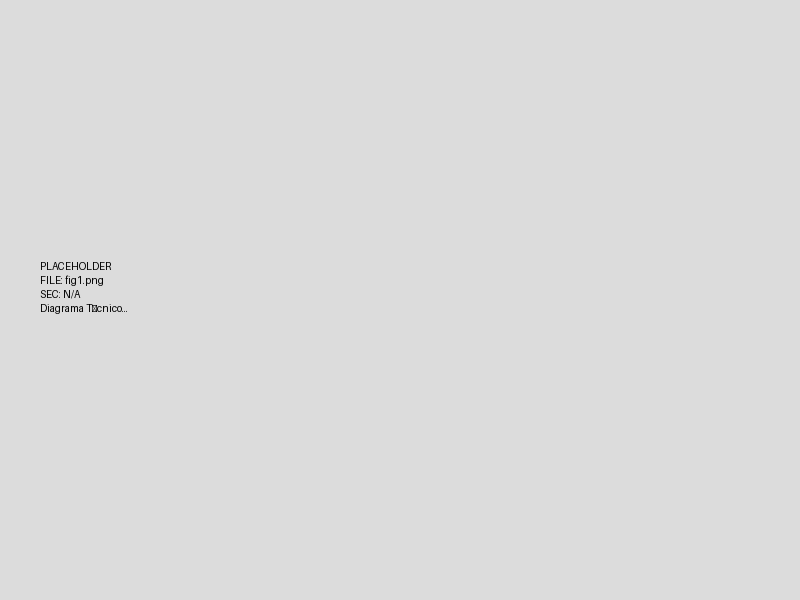
\includegraphics[width=\linewidth]{fig1.png}
\caption{Diagrama del pipeline propuesto de cloud masking y filtrado inteligente on-board. Se ilustran las etapas de adquisición multi-espectral, inferencia eficiente, decisión de downlink y flujos de datos selectivos.}
\label{fig:pipeline}
\end{figure}

En las siguientes secciones se detalla primero el estado del arte, luego las arquitecturas propuestas, las técnicas de optimización de inferencia, los resultados experimentales y, finalmente, las implicaciones operacionales y direcciones futuras.